\documentclass[12pt]{article}
\usepackage[english]{babel}
\usepackage[utf8x]{inputenc}
\usepackage{amsmath}
\usepackage{graphicx}
\usepackage[colorinlistoftodos]{todonotes}

\usepackage{subfigure}% Support for small, `sub' figures and tables
\usepackage{float} 
\usepackage{array}
\usepackage{url}
\usepackage{enumitem}

\usepackage{listings} % code listing
\usepackage{color}

\definecolor{dkgreen}{rgb}{0,0.6,0}
\definecolor{gray}{rgb}{0.5,0.5,0.5}
\definecolor{mauve}{rgb}{0.58,0,0.82}

\lstset{frame=tb,
    language=Java,
    aboveskip=3mm,
    belowskip=3mm,
    showstringspaces=false,
    columns=flexible,
    basicstyle={\scriptsize\ttfamily},
    numbers=none,
    numberstyle=\tiny\color{gray},
    keywordstyle=\color{blue},
    commentstyle=\color{dkgreen},
    stringstyle=\color{mauve},
    breaklines=true,
    breakatwhitespace=true,
    tabsize=3
}


\begin{document}
    
    \begin{titlepage}
        
        \newcommand{\HRule}{\rule{\linewidth}{0.5mm}} % Defines a new command for the horizontal lines, change thickness here
        
        \center % Center everything on the page
        
        %----------------------------------------------------------------------------------------
        %    HEADING SECTIONS
        %----------------------------------------------------------------------------------------
        
        \textsc{\LARGE Central Washington University}\\[1.5cm] % Name of your university/college
        \textsc{\Large CS530 High Performance Computing}\\[0.5cm] % Major heading such as course name
        \textsc{\large Spring 2019}\\[0.5cm] % Minor heading such as course title
        
        %----------------------------------------------------------------------------------------
        %    TITLE SECTION
        %----------------------------------------------------------------------------------------
        
        \HRule \\[0.4cm]
        { \huge \bfseries Lab1: Matrix Power Operation}\\[0.2cm] % Title of your document
        \HRule \\[1cm]
        
        %----------------------------------------------------------------------------------------
        %    AUTHOR SECTION
        %----------------------------------------------------------------------------------------
        
        \begin{minipage}{0.5\textwidth}
            \begin{flushleft} \large
                \emph{Student:}\\
                \begin{itemize}
                    \item Chao \textsc{Huang Lin} chao.huanglin@cwu.edu
                
                \end{itemize}
            \end{flushleft}
        \end{minipage}
        ~
        \begin{minipage}{0.45\textwidth}
            \begin{flushright} \large
                \emph{Professor:} \\
                Dr. Szilárd \textsc{VAJDA}\\ % Supervisor's Name
                Szilard.Vajda@cwu.edu
            \end{flushright}
        \end{minipage}\\[0.5cm]
        
        % If you don't want a supervisor, uncomment the two lines below and remove the section above
        %\Large \emph{Author:}\\
        %John \textsc{Smith}\\[3cm] % Your name
        
        %----------------------------------------------------------------------------------------
        %    DATE SECTION
        %----------------------------------------------------------------------------------------
        
        {\large \today}\\ % Date, change the \today to a set date if you want to be precise
        
        %----------------------------------------------------------------------------------------
        %    LOGO SECTION
        %----------------------------------------------------------------------------------------
        
        
\includegraphics[width=8cm]{CWU-Logo.png}\\[.5cm] % Include a department/university logo - this will require the graphicx package
        
        %----------------------------------------------------------------------------------------
        
        \vfill % Fill the rest of the page with whitespace
        
    \end{titlepage}
    \newpage
    \tableofcontents
    \newpage
    
    
    
    \section{Introduction}
    
    For this project, the power operation of the square matrix has been coded in C++ and Python, there are in total 4 different versions: 
    \begin{enumerate}[label=\arabic*)]
        \item C++ dynamic allocated double pointer matrix.
        \item C++ dynamic allocated linked list matrix.
        \item python ijk for loop matrix.
        \item python numpy library linalg.matrix\_power.
    \end{enumerate}
    The CPU running time of each version has been recorded, for the c++ versions we used four different methods:
        \begin{enumerate}[label=\arabic*)] 
    \item g++ gprof profiler: get the CPU spent time of each function.
    \item clock() function: compute the processor (CPU) time (linux).
    \item time function: work with wall time in second
    \item gettimeofday: work with wall time in microsecond
        \end{enumerate}
    For the python versions, we obtained the time using time.clock and time.time function from the time library, this library is using c time library. 
    %https://www.pythoncentral.io/measure-time-in-python-time-time-vs-time-clock/
    the time.clock function means different from windows and linux, on Windows means wall clock time and in linux time.clock means CPU processor time \cite{python.time}.
    In our case, the python codes have been run on a windows machine.
     
     \subsection{Time complexity}
    If we analyze the square matrix power expressed as  $ m^n $, where $m$ denotes the size of $mxm$ matrix, and $n$ denotes the power of the matrix.
    We can obtain the time complexity equation illustrated in equations \ref{eq:time1} and \ref{eq:time2}
     
     \begin{equation} \label{eq:time1}
      [m^2*[(m-1)+m)]]*(n-1)
     \end{equation}
    
    The value $[(m-1)+m)]$ represents the operation times when we do matrix multiplication, where  $(m-1)$ is the number of sum times, and $m$ is the number of the multiplication times in each of the $m^2$ matrix elements. The $(n-1)$ represents the numbers of matrix multiplication required when it is elevated to the power of $n$. This equation \ref{eq:time1} can be simplified to equation \ref{eq:time2}.
      
    \begin{equation} \label{eq:time2}
    [2m^3-m^2]*(n-1)
    \end{equation} 
     
    \section{Computer Specification}
     
    For this Lab, we used a Microsoft Surface Pro 3 which has the following specification: Core i7-4650U CPU 1.7GHz 2.3GHz with 8 GB of RAM.
    
    The C++ codes have been run on docker where 2 CPUs and 2GB of RAM was assigned. The Docker image was from professor Szilard "szilardvajda/ubuntu\_cs470"
    
    
    \section{Method}
     We have implemented a specific class in c++ for each solution, the matrix double pointer solution is declared in matrix\_double\_pointer class displayed in the listing \ref{list:mdp}, and the matrix linked list solution is declared in the listing \ref{list:mll}.
    
    \begin{lstlisting}[language=c++, caption={matrix\_double\_pointer class}, label={list:mdp}]

class matrix_double_pointer
{
int m; // mxm matrix
long double **matrix;

public:
matrix_double_pointer(int m); // constructor
matrix_double_pointer(const matrix_double_pointer& a); // copy constructor for return
~matrix_double_pointer(); //destructor
void init_identity(); //init identity matrix
void init(long double x); //init matrix all with x
void init_rand(); //init matrix with pseudo random 
void print_values();
void print_memory_address();
matrix_double_pointer operator* (const matrix_double_pointer& a);
matrix_double_pointer operator^ (int n);
matrix_double_pointer& operator= (const matrix_double_pointer& a); // assigment
long double** get_matrix();
};
    
    \end{lstlisting}
    To implement classes that work with pointers, we must take some special consideration \cite{class.pointer}. These classes should have:
    \begin{itemize}
        \item a destructor (to delete the allocated memory).
        \item a copy constructor (to copy the object when is returned, passed as parameter or initialization from another object of the same class). 
        \item an overloaded operator = (to assign or copy the data to another object).  
    \end{itemize}
     
From listing \ref{list:mdp} and \ref{list:mll} we can observe that all these 3 member functions are implemented. In addition, we have overload the operator $\wedge$ to get the matrix power in a more intuitive way. 
      
    
    %http://pages.cs.wisc.edu/~hasti/cs368/CppTutorial/NOTES/CLASSES-PTRS.html
    \begin{lstlisting}[language=c++, caption={matrix\_linked\_list class}, label={list:mll}]    
    struct node
    {
        long double data;
        int j;
        node *right;
    };
    struct head_node
    {
        long double data;
        int i;
        int j;
        node *right;
        head_node *down_head_node;
    };
    
    class matrix_linked_list
    {
        int m; // mxm matrix
        head_node *main_head_node;
        head_node *current_head_node; //for get_value_loop_opt()
        node *current_node; //for get_value_loop_opt()
        head_node *current_head_node_add; // add_value_loop_opt()
        node *current_node_add; // for add_value_loop_opt()
        
        void start_using_get_value_loop_opt();
        long double get_value_loop_opt(int i, int j); // optimized version of get_value (make the loop faster using temp node address)
        void add_value_loop_opt(long double value, int i, int j); // // optimized version of add_value (make the loop faster using temp node address)
        
        public:
        matrix_linked_list(); // constructor 
        matrix_linked_list(int m); // constructor 
        matrix_linked_list(const matrix_linked_list& a); // copy constructor for return
        ~matrix_linked_list(); //destructor
        void load(long double **matrix, int m); // receive square matrix and size mxm
        void delete_all_node();
        void print_values();
        void print_values_ij();  //print the data and also print i,j 
        void set_main_head_node(head_node *main_head_node);
        long double get_value(int i, int j);
        void add_value(long double value, int i, int j); // add value to the existing i,j if not -> create new node
        matrix_linked_list operator^ (int n);
        matrix_linked_list& operator= (const matrix_linked_list& a); // assigment
    };
\end{lstlisting}    

To create a linked list matrix, we used two different data structure: a head\_node struct for the elements which is located at the first column of the matrix, this head node contains the data, i, j values and two pointers: a node pointer to the next right node, and a head\_node pointer to the next down head node. Another data structure is a node structure which contains the data, j value and a node pointer to the next right node.

In this class we implemented two extra functions: add\_value\_loop\_opt() and get\_value\_loop\_opt() that  make the matrix multiplication faster, these function are optimized function of add\_value() and get\_value() that must be used inside a loop, more details will be explained in the subsection \ref{subsec:opt}.

    \section{Results}

    
Two solutions of C++ matrix power operation result are displayed in the listing \ref{list:result}, we can observe that the $m=3$ and $n=3$ operation was calculated correctly, also we can notice from the listing that in the linked list solution the memory is not allocated when the value equal to 0.
    \begin{lstlisting}[language=c++, caption={matrix power results}, label={list:result}]    
Input (m x m) matrix dimension m: 3
3
Input n from (m x m)^n: 3
3

matrix values // random double pointer matrix mxm
8:0:1:
0:3:1:
6:5:2:

matrix values (i,j) // random linked list matrix mxm
(0,0) 8 : ( ,2) 1 :
(1,1) 3 : ( ,2) 1 :
(2,0) 6 : ( ,1) 5 : ( ,2) 2 :

matrix values  // double pointer matrix power result m^n
620:65:95:
78:67:30:
570:150:115:

matrix values (i,j) // linked list matrix power result m^n
(0,0) 620 : ( ,1) 65 : ( ,2) 95 :
(1,0) 78 : ( ,1) 67 : ( ,2) 30 :
(2,0) 570 : ( ,1) 150 : ( ,2) 115 :
\end{lstlisting}    

    \subsection{Process Running Time}

    
First, we run two different solutions of matrix power operation with c++ codes simultaneously in 4 different tasks (fig. \ref{fig:run}) which each task consumes 50\% of each core (detected by docker). Then, we obtained the processing time from four different methods of running time calculution: g++ gprof profiler, clock() function, time() function and the gettimeofday() function, the results are shown in figure \ref{fig:cpptime}. 

    \begin{figure}[H]
    \centering
    
    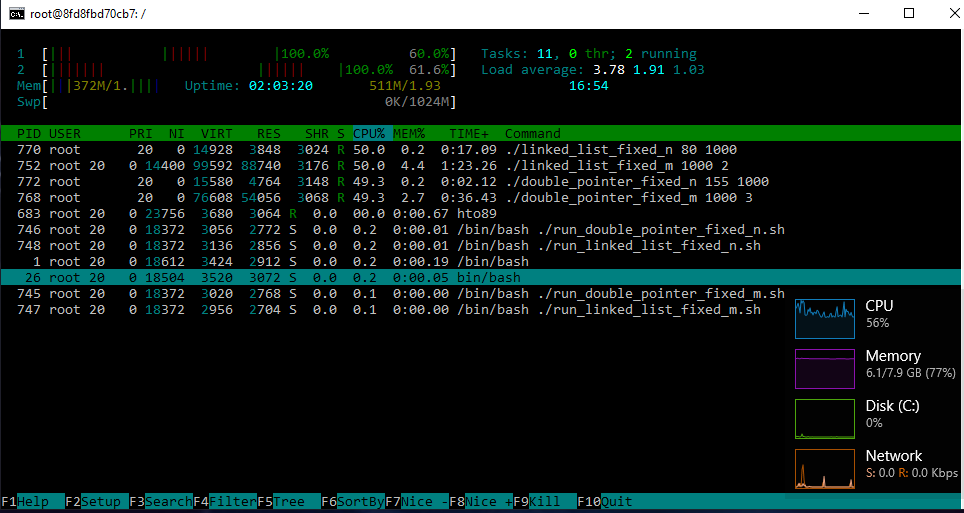
\includegraphics[width=\linewidth]{figures/run.png}
    
    \caption{Running the code in different thread} 
    \label{fig:run}
\end{figure}

As described above, the time() and getmeofday() work with wall time, this time may take longer than the processing time that the CPU assigned to a specific task because many tasks share the CPU resource. The clock() the time from profiling is actually CPU processing time, this gives us the time that the CPU used to run the program. For example, at the beginning of figure  \ref{fig:cpptime}  (a) the wall time (time and gettimeof day) is twice bigger than the clock time, this is because we started the 4 tasks simultaneously and each task consume 50\% of 1 core of the CPU, so the  resource of the core is shared by two tasks. This behavior can be observed in every sub-figure from figure \ref{fig:cpptime}. However, after some tasks finished, the core resource is released, so another task will take the resource, and this will change the previous relation between CPU clock time and wall time. Additionally, we can observe that at the end of figure \ref{fig:cpptime} (b) and (c) the CPU clock time is equal to wall time since at that moment each task was taking 100\% of each core of the CPU.

Another important aspect can be seen in figure \ref{fig:cpptime} (b) and (d), is that clock() time was very similar to profiling time, but when the processing time is bigger than 2000 the time from the g++ profiler become strange,  this seems to be that the time variable from g++ profile has some problem with overflow. Thus, in the following analysis, we will focus on the processing time calculated by the clock() function.
\begin{figure}[H]
    \centering
    
    \subfigure[Double Pointer fixed m]{     
        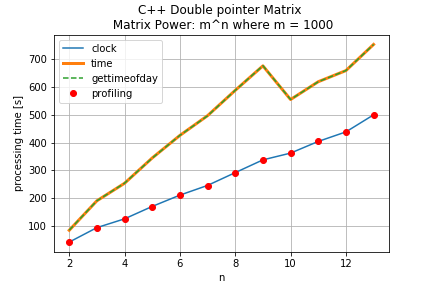
\includegraphics[width=0.47\linewidth]{figures/cpp_double_pointer_fixed_m.png}
    }
    \subfigure[Linked List fixed m]{     
        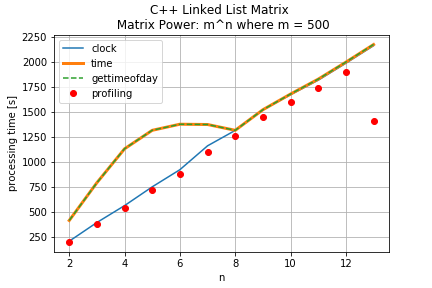
\includegraphics[width=0.47\linewidth]{figures/cpp_linked_list_fixed_m.png}
    }
    \subfigure[Double Pointer fixed n]{     
    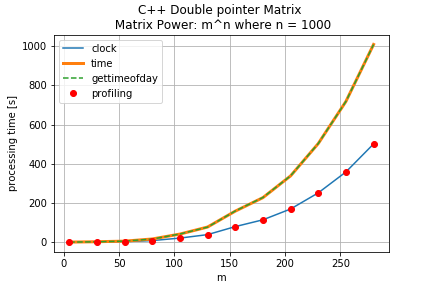
\includegraphics[width=0.47\linewidth]{figures/cpp_double_pointer_fixed_n.png}
    }
    \subfigure[Linked List fixed n]{     
    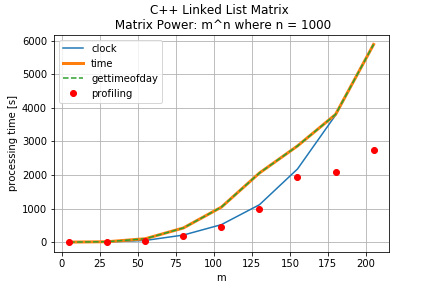
\includegraphics[width=0.47\linewidth]{figures/cpp_linked_list_fixed_n.png}
    }

    \caption{C++ Running Time Using Profiler and Clock} 
    \label{fig:cpptime}
\end{figure}

    The figures \ref{fig:cpptime} (a) and (b) show the double pointer solution and the linked list solution respectively, both have processed a matrix power operation with fixed m, we can observe that these figures follow a linear trend, this behavior is supported by the equation \ref{eq:time2} which shows a linear equation when we make the $m$ constant.
    In contrast, the figures \ref{fig:cpptime} (c) and (d) show the result of matrix power operation with fixed n, the graph seems to follow a polynomial behavior, this can also be demonstrated by the equation \ref{eq:time2} when we make the $n$ constant, the equation becomes polynomial function.

%Moreover, we can also observe from the figures that the calculated time from profiler very similar to the clock() function, is just a little smaller than the clock() function.

Additionally, the figures show that the double pointer matrix is much faster than the linked list, this is because that the double pointer matrix memory is contiguous in each row and the memory access can be faster. In contrast, for the linked list it needs to access  no contiguous memory location each time, also it requires memory allocation for each node in different time, and the memory deletion must be done separately for each node, and for the object based programming it need to copy each node when we use assignment operator (=) and copy constructor. All these factors make the linked list slower.

%https://stackoverflow.com/questions/5983059/why-is-a-linkedlist-generally-slower-than-a-list

The figure \ref{fig:python} follows the same pattern as described above. One observation is that the python for loop is tremendously slow because python is a scripting language. However, we can also observe from the graph that the numpy matrix\_power() function is extremely fast, even it is much faster than c++ solution, this is because that the numpy library is written in a very optimized c code \cite{numpy}.

\begin{figure}[H]
    \centering
    
    \subfigure[for loop fixed m]{     
        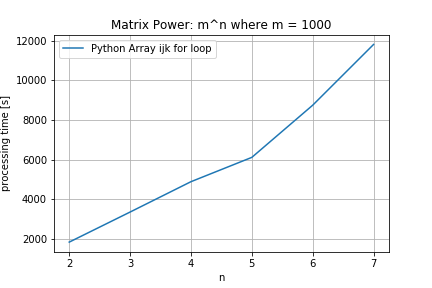
\includegraphics[width=0.47\linewidth]{figures/python_fixed_m.png}
    }
    \subfigure[numpy matrix\_power() fixed m]{     
        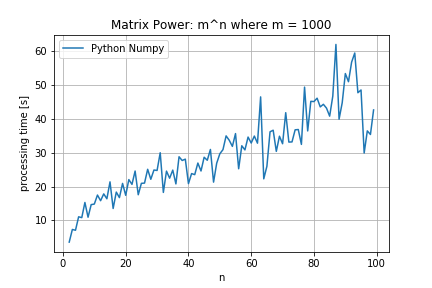
\includegraphics[width=0.47\linewidth]{figures/python_numpy_fixed_m.png}
    }
    \subfigure[for loop fixed n]{     
        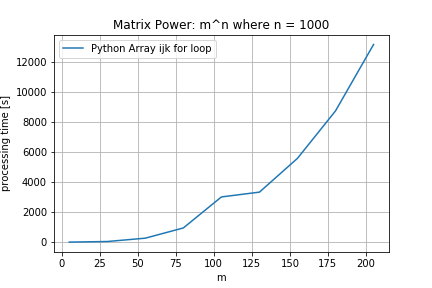
\includegraphics[width=0.47\linewidth]{figures/pyton_fixed_n.png}
    }
    \subfigure[numpy matrix\_power() fixed n]{     
        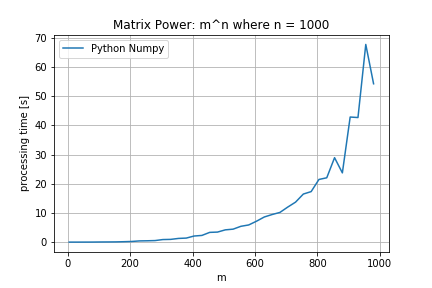
\includegraphics[width=0.47\linewidth]{figures/pyton_numpy_fixed_n.png}
    }
    
    \caption{Python Running Time Using time library} 
    \label{fig:python}
\end{figure}


%https://introcs.cs.princeton.edu/python/appendix_numpy/

\subsection{Profiler and Optimization}\label{subsec:opt}
For this project, we have used profiler, clock(), time() and gettimeofday()  functions to calculate the process running time, despite the overflow problem, the profiler method gave us a more detailed result, and this allows us to identify which function of the code is consuming more time. For example, the listing \ref{list:profile} shows us the profiling result of matrix power using linked list where $m=80$ and $n=1000$.  

\begin{lstlisting}[language=c++, caption={matrix\_double\_pointer class}, label={list:profile}, basicstyle=\tiny]

Flat profile:

Each sample counts as 0.01 seconds.
%   cumulative   self              self     total           
time   seconds   seconds    calls   s/call   s/call  name    
64.37    518.02   518.02 1022976000     0.00     0.00  matrix_linked_list::get_value(int, int)
34.78    797.90   279.88 511488000     0.00     0.00  matrix_linked_list::add_value(long double, int, int)
0.77    804.07     6.17        1     6.17   804.58  matrix_linked_list::operator^(int)
0.07    804.60     0.53                             matrix_linked_list::print_values_ij()
0.04    804.92     0.32     2004     0.00     0.00  matrix_linked_list::delete_all_node()
0.02    805.11     0.19     1000     0.00     0.00  matrix_linked_list::operator=(matrix_linked_list const&)
0.00    805.11     0.00        5     0.00     0.00  matrix_linked_list::~matrix_linked_list()
0.00    805.11     0.00        2     0.00     0.00  matrix_linked_list::matrix_linked_list(matrix_linked_list const&)
0.00    805.11     0.00        2     0.00     0.00  matrix_linked_list::matrix_linked_list()
0.00    805.11     0.00        1     0.00     0.00  _GLOBAL__sub_I__ZN21matrix_double_pointerC2Ei
0.00    805.11     0.00        1     0.00     0.00  __static_initialization_and_destruction_0(int, int)
0.00    805.11     0.00        1     0.00     0.00  matrix_linked_list::load(long double**, int)
0.00    805.11     0.00        1     0.00     0.00  matrix_linked_list::matrix_linked_list(int)
0.00    805.11     0.00        1     0.00     0.00  matrix_double_pointer::get_matrix()
0.00    805.11     0.00        1     0.00     0.00  matrix_double_pointer::init_rand()
0.00    805.11     0.00        1     0.00     0.00  matrix_double_pointer::matrix_double_pointer(int)
0.00    805.11     0.00        1     0.00     0.00  matrix_double_pointer::~matrix_double_pointer()

\end{lstlisting}

As displayed in listing \ref{list:profile}, the total processing time of the programa was 805.11 seconds, the operator $\wedge$ consumed 804.58 seconds per call, inside the operator $\wedge$  we have get\_value() function that consumed 518.02 seconds and add\_value() function that consumed 279.88 seconds.
Consequently, with this information we have performed some changes to improve the processing time in the linked list code, the performance of  these changes is displayed in figure \ref{fig:opt} :

\begin{enumerate}[label=\alph*)]
    \item Without any change, so the address of head\_node and node will reset in each loop iteration. 
    \item We keep the head\_node address of the previous loop in the get\_value() function.
    \item We keep the head\_node and the node addresses of the previous loop in the get\_value() function.
    \item We keep the head\_node and the node addresses of the previous loop in get\_value() and add\_value() function.
\end{enumerate}


we can see clearly how these changed made the processing time of the program faster.

\begin{figure}[H]
    \centering
    
    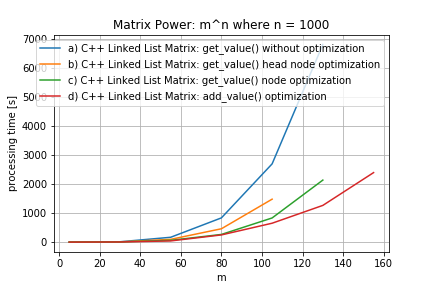
\includegraphics[width=0.7\linewidth]{figures/cpp_linked_list_fixed_n_optimization.png}
    
    \caption{C++ linked list running time (clock) after applying changes} 
    \label{fig:opt}
\end{figure}

    
    \section{Conclusion}
    In conclusion, we have implemented four versions of matrix multiplication solution, two in c++ and two in python, we found that in c++ the double pointer matrix was faster than the linked list one, because in the linked list version there is a lot of memory access and allocation work, and we also noticed that the python ijk loop was much slower than c++ solutions, this is because python is a scripting language. However, the version with matrix\_power() from numpy library performed much faster than the c++ solutions since the numpy library is coded in high optimized c code. 
    
    Moreover, we have compared the different meaning of timing functions, then we found that clock() time and profiling time was better since it calculates the CPU processing time, and we detected a potential bug in g++ profiling related with overflow.
    
    In addition,  we have demonstrated with figures that the behavior of the processing time follow the equation trend of the equation: $[2m^3-m^2]*(n-1)$. 
    
    Finally, we consider that the profiling method is very useful for coding optimization, and we were able to improve the running time linked list with the help of profiling.
    \bibliographystyle{unsrt}
    \bibliography{references}
\end{document}